\chapter[Présentation de l’organisme]{Présentation de l’organisme d’accueil et cadre général du projet}

\section{Introduction}

Le Projet de Fin d’Études constitue une étape importante dans le parcours du Master en Data Science et Sécurité des Systèmes d’Information. Il permet de mobiliser les connaissances acquises durant la formation autour d’un projet concret, combinant analyse, conception, développement logiciel et validation technique.

Le présent projet, intitulé \textbf{Virtual FabLab}, s’inscrit dans le contexte de la transformation numérique des environnements de fabrication et d’apprentissage. Il vise à proposer une plateforme web permettant de visualiser un FabLab virtuel, de gérer ses machines, de simuler des opérations de fabrication numérique et d’exploiter des données IoT simulées pour la supervision intelligente.

Ce chapitre présente l’organisme d’accueil, le cadre général du projet, la problématique traitée ainsi que les objectifs poursuivis.

\section{Présentation de l’ENSA Béni Mellal}

L’École Nationale des Sciences Appliquées de Béni Mellal, désignée dans ce rapport par ENSA BM, est un établissement public d’enseignement supérieur relevant de l’Université Sultan Moulay Slimane. Elle participe à la formation de profils scientifiques et technologiques capables de répondre aux besoins du marché dans les domaines de l’ingénierie, de l’informatique, de la data science, des réseaux et des systèmes d’information.

L’ENSA BM offre un environnement académique favorable à l’apprentissage par projet, à l’innovation et à l’expérimentation technique. Dans ce cadre, les projets de fin d’études occupent une place essentielle, car ils permettent aux étudiants de confronter leurs compétences à des problématiques réelles ou proches du réel.

\section{Missions et formations}

\subsection{Missions de l’établissement}

Les missions principales de l’ENSA BM peuvent être résumées comme suit :

\begin{itemize}
    \item assurer une formation scientifique et technique de haut niveau ;
    \item développer les compétences en ingénierie, en informatique et en technologies numériques ;
    \item encourager la recherche appliquée, l’innovation et l’esprit d’initiative ;
    \item préparer les étudiants à l’intégration professionnelle et à la conduite de projets complexes ;
    \item contribuer au développement régional et national à travers la formation de profils qualifiés.
\end{itemize}

\subsection{Formations proposées}

L'École Nationale des Sciences Appliquées de Béni Mellal propose des formations d'ingénieurs orientées vers les sciences appliquées, les technologies et l'ingénierie. Ces formations visent à développer des compétences scientifiques et techniques adaptées aux besoins du monde professionnel.

Les domaines de formation couvrent notamment :

\begin{itemize}
    \item l'informatique et les technologies numériques ;
    \item les systèmes embarqués et connectés ;
    \item les télécommunications ;
    \item les systèmes industriels ;
    \item l'ingénierie et les sciences appliquées.
\end{itemize}

Dans ce contexte technologique, l'ENSA de Béni Mellal constitue un environnement adapté à la réalisation du projet Virtual FabLab, qui intègre le développement web, la simulation 3D, les technologies IoT et l'exploitation des données.

\section{Organigramme de l’établissement}

L’organisation de l’ENSA BM repose sur une structure administrative et pédagogique permettant d’assurer le suivi des formations, l’encadrement des étudiants et la gestion des activités académiques.

\begin{figure}[H]
\centering
\IfFileExists{images/organigrame.png}
{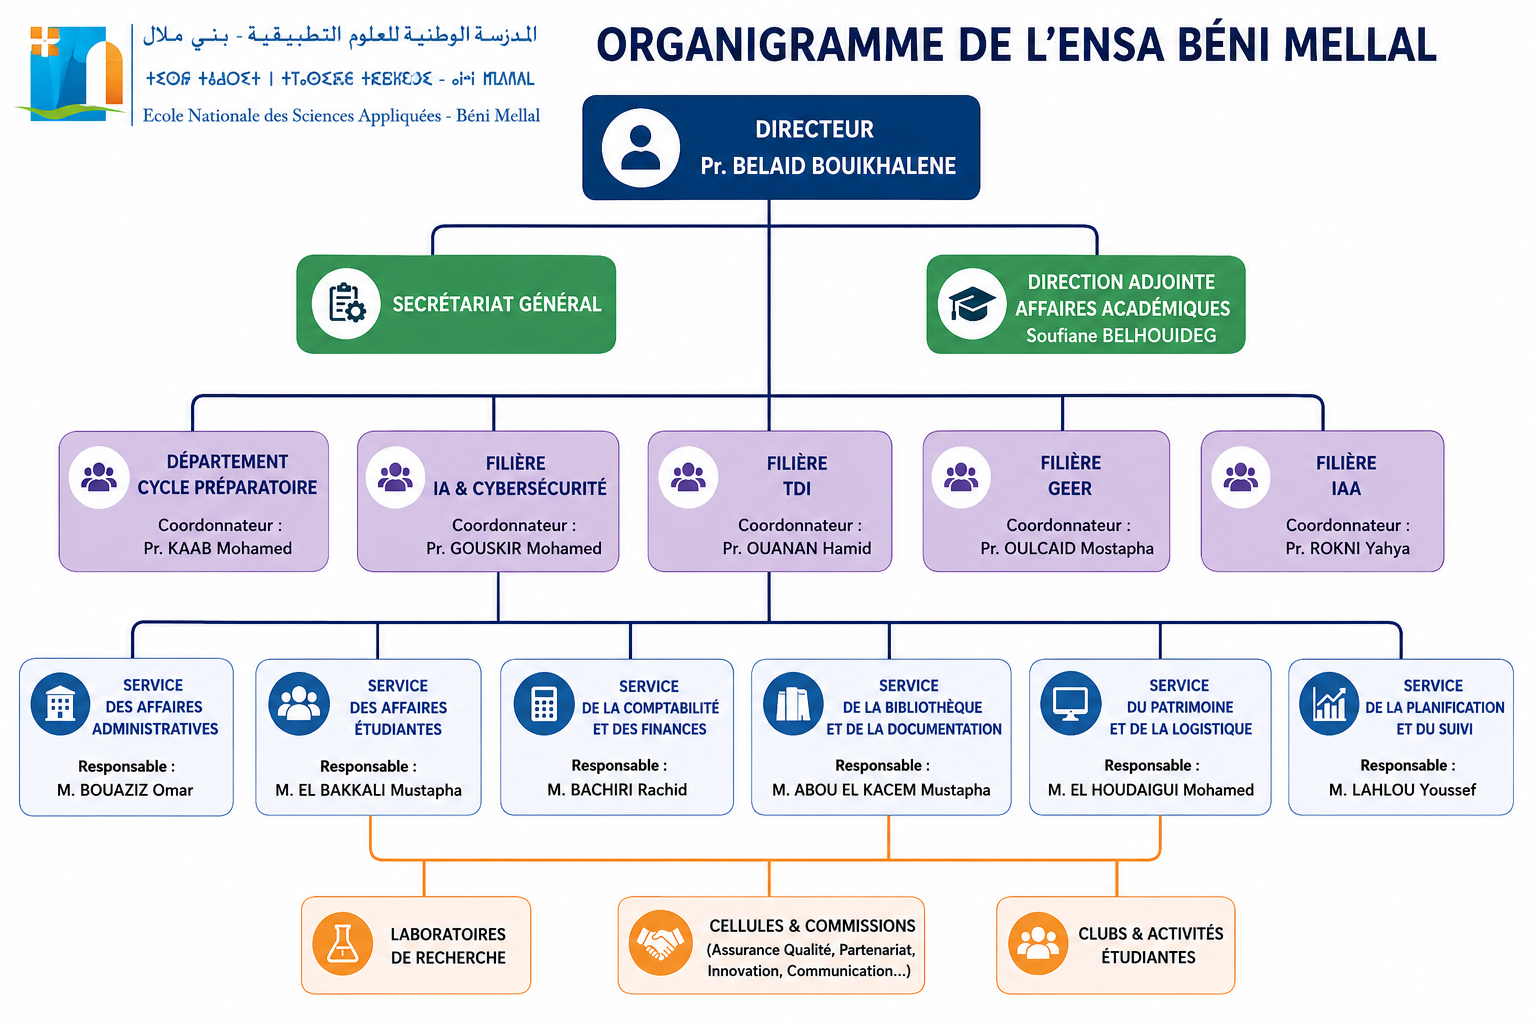
\includegraphics[width=0.95\textwidth]{images/organigrame.png}}
{\fbox{\parbox[c][5cm][c]{0.85\textwidth}{\centering Emplacement réservé pour l’organigramme de l’établissement\\\texttt{images/organigrame.png}}}}
\caption{Organigramme de l’ENSA Béni Mellal}
\label{fig:organigramme-ensa}
\end{figure}

La figure \ref{fig:organigramme-ensa} présente l’organisation générale de l’établissement. Cette structure permet de situer le projet dans son environnement académique et de comprendre le cadre institutionnel dans lequel il a été réalisé.

\section{Contexte du stage}

Le projet a été réalisé dans un contexte académique orienté vers l’innovation numérique et l’Industrie 4.0. Les FabLabs constituent aujourd’hui des espaces importants pour l’apprentissage pratique, le prototypage rapide et la fabrication numérique. Ils mettent à disposition des machines telles que les imprimantes 3D, les machines CNC ou les découpeuses laser.

Cependant, l’accès à ces équipements peut être limité par plusieurs contraintes : disponibilité des machines, besoin de présence physique, difficulté de supervision à distance et absence d’outils unifiés permettant de relier gestion, simulation et analyse de données.

Dans ce contexte, la création d’un FabLab virtuel représente une réponse pertinente. Elle permet de préparer les utilisateurs avant l’utilisation réelle des machines, de simuler des trajectoires de fabrication et d’introduire une couche de supervision intelligente fondée sur les données. Les données utilisées dans cette version sont simulées afin de valider l’architecture, les flux MQTT, le monitoring et le module d’analyse. La plateforme reste conçue pour être connectée ultérieurement à des capteurs réels.

\section{Problématique}

Les FabLabs traditionnels reposent principalement sur une interaction physique avec les équipements. Cette approche est utile pour l’apprentissage pratique, mais elle présente certaines limites dans un contexte pédagogique moderne. Les étudiants ne disposent pas toujours d’un moyen simple pour visualiser les machines, tester un fichier de fabrication ou consulter l’état des équipements avant une séance.

Par ailleurs, les machines de fabrication numérique produisent ou pourraient produire des données de fonctionnement telles que la température, la vibration, la durée d’utilisation, la vitesse du moteur ou les erreurs signalées. Ces données sont précieuses pour la supervision et la maintenance, mais elles restent souvent peu exploitées dans un cadre académique. Dans la version réalisée, ces mesures ne proviennent pas encore de capteurs physiques : elles sont générées par un simulateur MQTT afin de tester les traitements et les interfaces dans des conditions contrôlées.

La problématique du projet peut donc être formulée ainsi :

\begin{center}
\textit{Comment concevoir et réaliser une plateforme virtuelle permettant de gérer un FabLab, de simuler ses machines et d’exploiter des données IoT simulées pour la supervision intelligente et la maintenance prédictive ?}
\end{center}

\section{Objectifs du projet}

L’objectif principal du projet est de concevoir et développer une plateforme web nommée \textbf{Virtual FabLab}, intégrant la gestion des utilisateurs et des machines, la visualisation 3D, la simulation de fichiers de fabrication et l’exploitation de données IoT simulées.

Les objectifs spécifiques sont les suivants :

\begin{itemize}
    \item mettre en place une interface web moderne destinée aux étudiants et aux administrateurs ;
    \item permettre l’inscription, l’authentification et la gestion des profils utilisateurs ;
    \item gérer les machines du FabLab, leurs types, leurs états et leur positionnement dans l’espace 3D ;
    \item offrir un système de réservation des machines avec validation administrative ;
    \item construire une scène 3D interactive représentant le FabLab et ses équipements ;
    \item simuler le comportement d’une imprimante 3D et d’une machine CNC à partir de fichiers G-code ou NC ;
    \item intégrer une télémétrie simulée transmise via MQTT ;
    \item analyser les données simulées afin de détecter les anomalies et d’estimer l’état de santé des machines ;
    \item classifier les intentions administrateur liées à la supervision et à la maintenance ;
    \item proposer un Copilote IA d’aide à la décision réservé à l’administrateur ;
    \item afficher les indicateurs de supervision dans un tableau de bord administrateur.
\end{itemize}

\section{Présentation générale du Virtual FabLab}

La plateforme Virtual FabLab est conçue comme une application web complète reposant sur une architecture frontend/backend. Le frontend assure l’expérience utilisateur, la visualisation du laboratoire virtuel, les interfaces de réservation, les écrans administrateur et les vues de simulation. Le backend fournit les API, la persistance des données, l’authentification, la gestion des rôles, la réception des données MQTT et les services d’analyse.

La solution réalisée couvre plusieurs modules complémentaires :

\begin{itemize}
    \item un module d’authentification basé sur des jetons JWT ;
    \item un module de gestion des utilisateurs et des droits d’accès ;
    \item un module de gestion des machines et de leurs emplacements dans le FabLab virtuel ;
    \item un module de réservation avec suivi des demandes ;
    \item un module de visualisation 3D du laboratoire ;
    \item un module de simulation G-code pour imprimante 3D et CNC ;
    \item un module MQTT permettant l’ingestion de télémétrie simulée ;
    \item un module Data Science et IA pour la détection d’anomalies, le score de santé, l’estimation indicative du risque de maintenance, la classification d’intentions et le Copilote IA d’aide à la décision.
\end{itemize}

\begin{figure}[H]
\centering
\IfFileExists{images/vue_generale_virtual_fablab.png}
{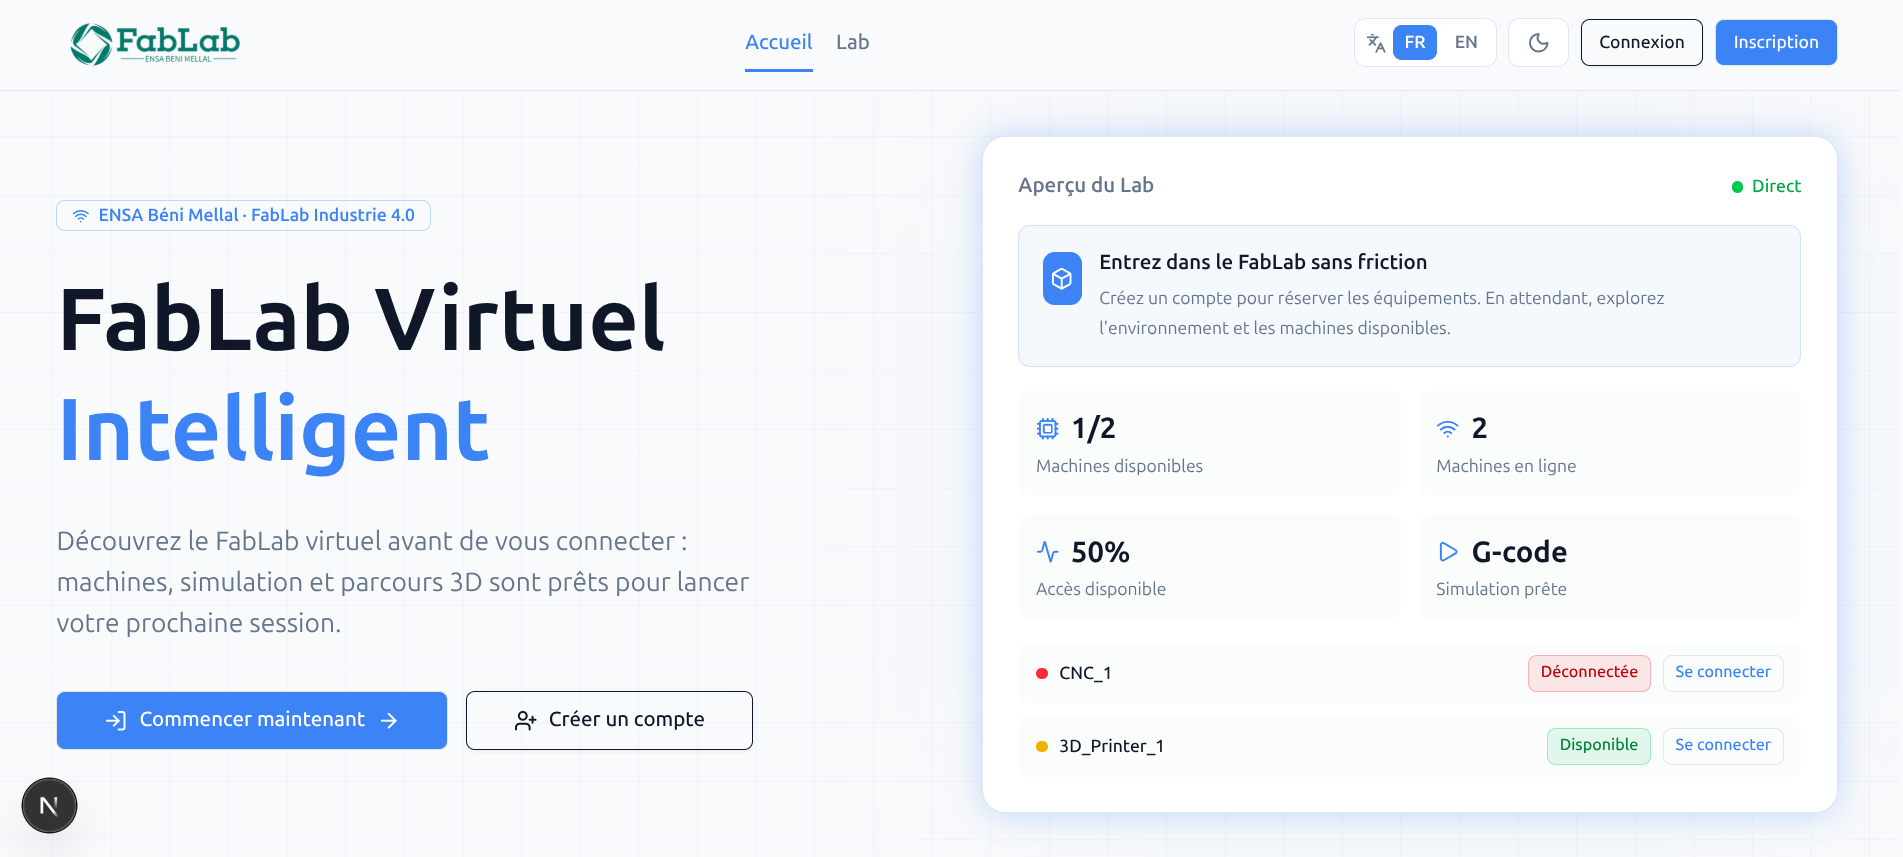
\includegraphics[width=0.9\textwidth]{images/vue_generale_virtual_fablab.png}}
{\fbox{\parbox[c][5cm][c]{0.85\textwidth}{\centering Emplacement réservé pour une vue générale de la plateforme\\\texttt{images/vue\_generale\_virtual\_fablab.png}}}}
\caption{Vue générale prévue de la plateforme Virtual FabLab}
\label{fig:vue-generale-virtual-fablab}
\end{figure}

\section{Conclusion}

Ce chapitre a présenté l’organisme d’accueil, le contexte général du projet, la problématique ainsi que les objectifs de la plateforme Virtual FabLab. Le projet se positionne à l’intersection du développement web, de la simulation 3D, de l’IoT et de la Data Science.

Le chapitre suivant sera consacré à l’analyse des besoins et à la conception du système. Il présentera les acteurs, les fonctionnalités attendues, l’architecture générale, les modules de la plateforme ainsi que les technologies retenues pour la réalisation.
